\chapter{Introduction}

OptoFidelity TOUCH product is a robotics platform for testing smart devices, automotive infotainment systems and other consumer electronics with focus on touch screen testing. These devices are commonly referred to as Device Under Test (DUT) in this document. The standard hardware consists of multi-axis robot capable of fully synchronous closed-loop control and a PC and other accessories required to control the system. This user manual focuses on the software that is used to control TOUCH systems. This chapter gives a general overview of the software and each component is treated in more detail in dedicated chapters.

The most common robot type is Synchro finger robot as shown in Figure \ref{fig:synchro_robot}. It has three linear axes to enable movement across the workspace and Synchro finger tool which can rotate around the vertical axis, move two fingers along axis that is perpendicular to the rotation axis and even move the two fingers separately along vertical axis using voice coil actuators. All the axes can be controlled synchronously with the software to create many types of movements that are useful when testing smart devices. A camera is attached to the robot to enable positioning DUTs and tips based on machine vision and to perform functional testing of DUTs. It is possible to position multiple DUTs and tip slots in the workspace and the system is able to change tips automatically.

\begin{figure}[!h]
	\centering
	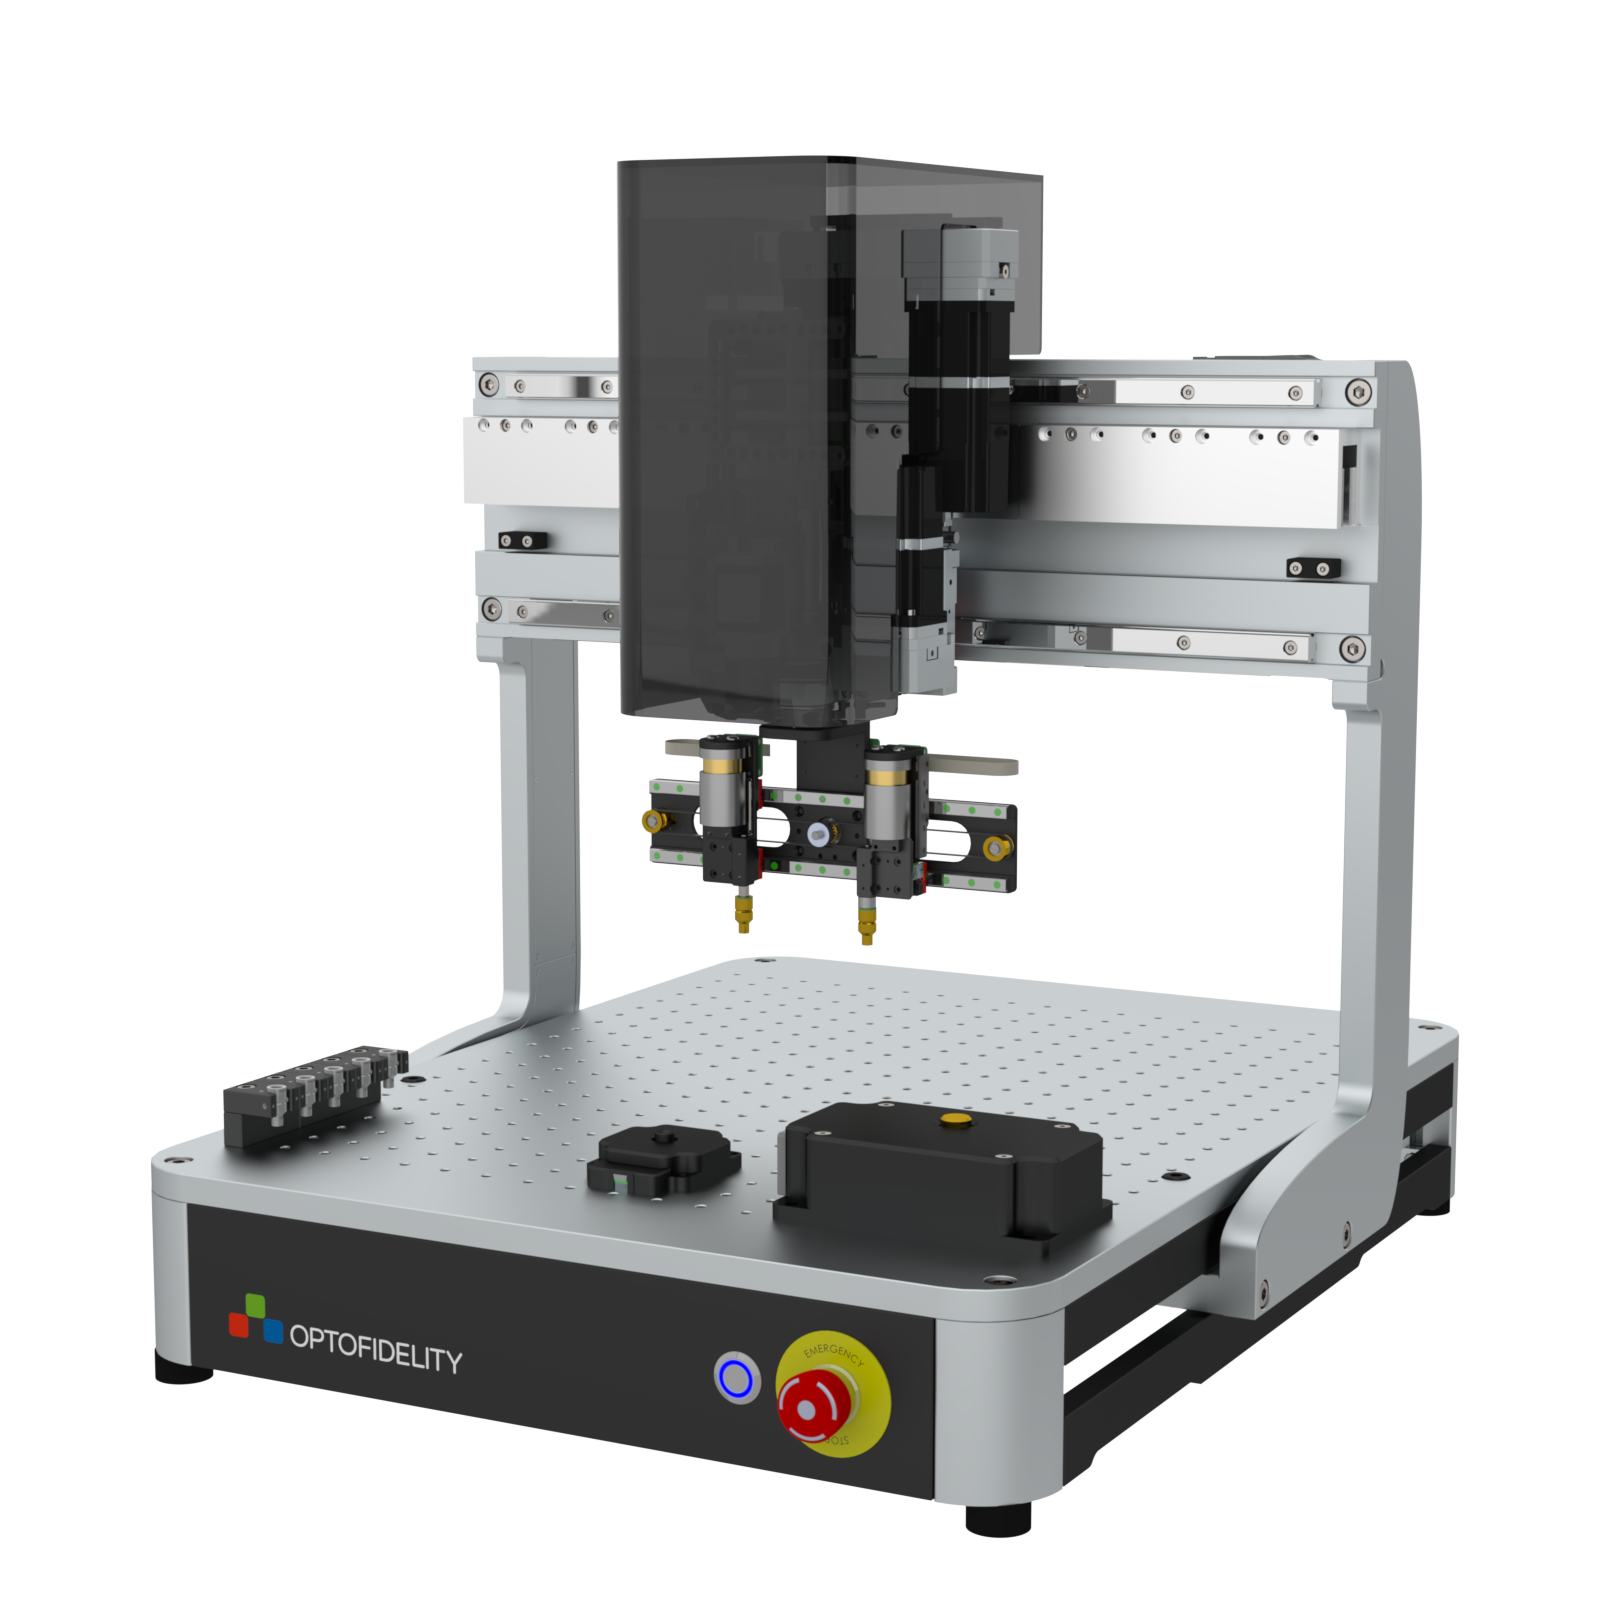
\includegraphics[width=8cm]{synchro_robot.png}
	\caption{Robot with Synchro finger tool. In the workspace from left to right are finger tip rack, Audit gauge for finger and camera offset calibration and Force calibration unit.}
	\label{fig:synchro_robot}
\end{figure}

\section{Software overview}

The core part of the software is TnT (Touch and Test) Server. It is a native stand-alone application that is distributed for Windows and Macos operating systems and installed on a dedicated delivery PC. The PC is further connected to a robot axis controller and other devices such as cameras, calibration tools and so on. The axis controller is typically OptoFidelity proprietary Optomotion controller but also other controllers may be used depending on robot type. Optomotion controls the individual axes of the robot and can be further used for controlling IO channels and trigger signals if necessary for the delivered system. These relations are shown in Figure \ref{fig:server_sw}.

\begin{figure}[!h]
	\centering
	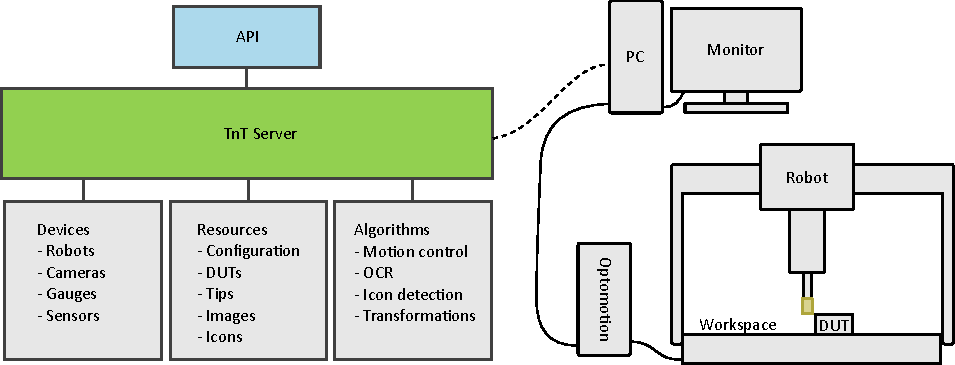
\includegraphics{server_sw.pdf}
	\caption{Illustration of TnT Server, control PC, Optomotion and robot.}
	\label{fig:server_sw}
\end{figure}

On a more detailed level, TnT Server implements drivers for controlling various devices such as robots, cameras, detectors and sensors. It also stores various resources that can be created at runtime and stored to disk for future use. These resources include system configuration, DUT positioning data, tip dimensions, images (from cameras or other sources) and icon shape models. TnT Server also implements algorithms that use the devices and resources. These include robot motion planning and motion control, optical character recognition (OCR), icon detection and transformations between different coordinate systems. These transformation are essential part of the entire system as the resources and devices (e.g. robots and DUTs) usually have specific position and orientation in the 3D space and need to be treated in relation to each other. The DUT coordinate system is very useful in most typical use cases. For example, when user wants to write scripts where gestures are performed on DUT, the DUT needs to be positioned in the workspace only once and then the local DUT coordinates can be used in scripting to keep things simple.

TnT Server, as the name implies, is actually an HTTP server. Once it has successfully initialized, it will just wait for incoming requests via REST API. These requests can for example move the robot to given position, return current robot position, create new DUTs, find an icon from existing DUT using a camera, just to name a few.

\begin{figure}[!h]
	\centering
	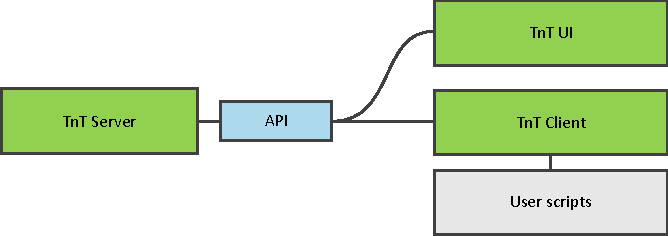
\includegraphics{server_client.pdf}
	\caption{TnT Server and other software components communicate via REST API.}
	\label{fig:server_client}
\end{figure}

TnT Server is capable of controlling the entire system, but usually it is not very accessible as such. Users are provided with more productive ways of using the API. The most basic way is by use of TnT Client. This is a client side implementation of the API in some specific programming language, most typically Python. It documents what the API can do and what parameters can be provided. Users can create virtually any type of test scripts based on TnT Client. It is also advised to use TnT Client instead of the REST API directly as OptoFidelity aims to keep breaking changes in TnT Client minimal in future versions.

The use of Python TnT Client is very easy. It is a Python package with minimal dependencies and can be ran on the delivery PC or remote PC in normal Python interpreter. Example below shows how to move robot effector 50 mm along the workspace  x-axis:

\begin{lstlisting}[language=Python]
from tntclient.tnt_client import TnTClient

# Create client object. By default connects to localhost.
client = TnTClient()

# Create client object to control the default robot configured in TnT Server.
robot = client.robot("Robot1")

# Move robot from current position 50 mm along the workspace x-axis.
robot.move_relative(x=50)
\end{lstlisting}

More examples and the client API reference can be found inside the provided TnT Client Python package.

For performing the most typical tasks such as positioning DUTs, adding tips and teaching icons, there is TnT UI. It is also a stand-alone application that is typically run on the delivery PC and it interfaces with TnT Server via the API. In principle the UI could be run on a remote PC that is connected to the delivery PC via a network. The interface between TnT Server and other software components is shown in Figure \ref{fig:server_client}. See \autoref{ch:ui} for more detailed description of TnT UI features.
